\section{Face and person detection and tracking}
\label{subsec:face_tracking}
In the pursuit of refining character representation within the MovieGraphs dataset~\cite{moviegraphs}, we initiate a comprehensive process of face and person detection across every movie scene. Leveraging advanced deep learning methodologies, we employ the Multi-Task Cascaded Convolutional Neural Networks (MTCNN)~\cite{mtcnn} for face detection and Cascade-RCNN pretrained on cast annotations from MovieNet~\cite{movienet} for person detection.

\begin{figure}[t]
\centering
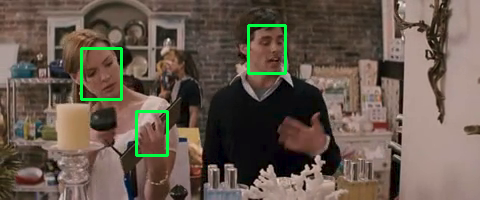
\includegraphics[width=0.49\linewidth]{Figures/falsePositive_face_1.png}
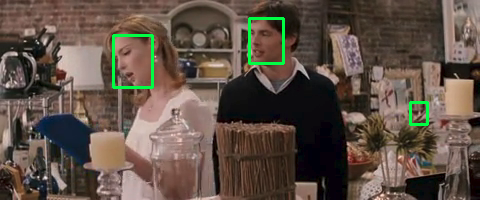
\includegraphics[width=0.49\linewidth]{Figures/falsePositive_face_2.png}
\vspace{-2mm}
\caption{False positive face detections by MTCNN~\cite{mtcnn} given the entire frame at once with threshold set to 0.95. The detector still predicts incorrect face bounding boxes.}
\vspace{-4mm}
\label{fig:falsePositiveFaces}
\end{figure}

Figure \ref{fig:falsePositiveFaces} shows the false positive bounding boxes predicted by MTCNN~\cite{mtcnn} detector when given the entire frame. MTCNN~\cite{mtcnn} is sensitive to threshold and using using higher threshold does not guarantee perfect face detection.

\begin{figure}[t]
\centering
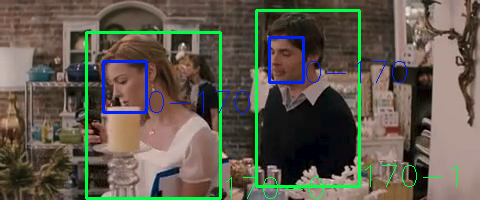
\includegraphics[width=0.49\linewidth]{Figures/faceInsidePersonBox_1.png}
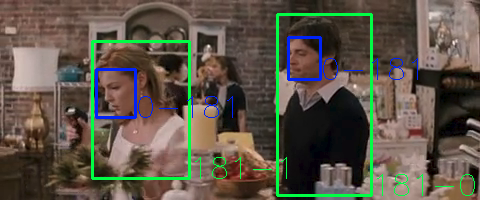
\includegraphics[width=0.49\linewidth]{Figures/faceInsidePersonBox_2.png}
\vspace{-2mm}
\caption{Confined face detections within the person bounding boxes. This allows us to have a correspondence between the person and face detections and ensemble of both the models considerably reduces the false positives.}
\vspace{-4mm}
\label{fig:facesInsidePersonBox}
\end{figure}

To mitigate this issue, we undertake a two-step process to seamlessly integrate person detections. First, we utilize the Cascade-RCNN to compute person bounding boxes within each movie scene. Subsequently, we extract face detections confined within these person bounding boxes, establishing a crucial mapping between face and person detections. Figure \ref{fig:facesInsidePersonBox} shows the face detections confined within the person bounding boxes. This considerably resolves the issue of incorrect face detections.
In the event of multiple faces coexisting within a single person bounding box, our methodology prioritizes accuracy by selecting the face with the highest detection probability. This ensures that the ensuing face detections maintain fidelity to the most salient facial representation within the confined space.

The resulting face and person bounding boxes are subjected to tracking mechanisms for continuous identity mapping across frames. To achieve this, we implement the Kalman-filter based Simple Online and Realtime Tracking (SORT) algorithm~\cite{sort}, enabling real-time tracking of these bounding boxes. Importantly, our approach establishes a direct mapping between face and person tracks, sharing the same track ID for seamless coordination between the two modalities. Figure \ref{fig:sortTrackedDetections} shows the consistent track id for multiple characters in different frames within the same shot of a movie scene. The tracking ids however gets updated at the shot boundaries. We move on to the next step to establish the character mapping across shots within the movie scene.

\begin{figure}[t]
\centering
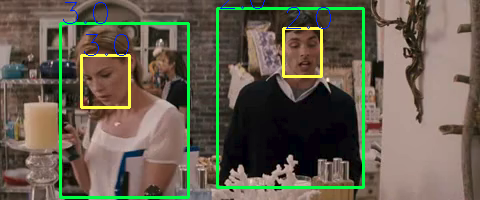
\includegraphics[width=0.49\linewidth]{Figures/sort_tracked_detections_2.png}
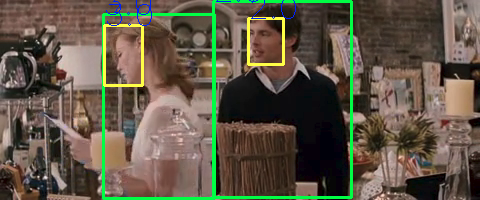
\includegraphics[width=0.49\linewidth]{Figures/sort_tracked_detections_1.png}
\vspace{-2mm}
\caption{Character detections with consistent track IDs across frames for both the actors. Our detection and tracking pipeline results in a consistent and reliable character tracks within a shot of a movie scene.}
\vspace{-4mm}
\label{fig:sortTrackedDetections}
\end{figure}
